\chapter{評価}
複数タスクにかかる所要時間に対し被験者の予測とADLoggerの予測の差異を比較した上で,
ADLogger導入によって,行動・意識の変容が生じるかどうか評価する.
本章ではまず評価概要を説明し,実験結果を示す.最後に,評価実験から得られた結果をもとに考察を行う.

\section{評価実験の概要}
本研究における評価実験の概要を述べる.はじめに,評価実験を行う目的を説明する.
ついで,評価実験を行う手順について説明する.

\subsection{評価の目的}
本研究では,複数タスクにかかる所要時間の予測に関して被験者の予測とADLoggerの予測の差異を比較する事,
ADLogger導入によって,時間管理に対する苦手意識・行動への変化が起こる事を目的としている.

\subsection{実験評価手法}
今回の評価実験では,被験者に時間の長さを教示し,その長さを産生させる時間産生法\cite{Oguro1961}\cite{Tayama2018}を参考にし3回の計測実験を慶應義塾大学の学生男女30名(目標)に対し1ヶ月実施した.
始めに,被験者は事前に各自保持しているiPhoneにADLoggerをインストールして貰う.
インストール後,実験で用いたい日常生活動作を3タスク程度,各タスク所要時間5分から15分程度を決定し,タスク名,タスク毎の必要時間予測,タスクを連続で行った時の必要時間予測をADLoggerのアンケート画面から回答する.後日zoom\cite{zoom}を用いながら実際に行動して貰い実測値を計測する.

その後,被験者自身が実験用に定めた動作3タスク分に関しては被験者は該当するタスクを日常生活で行う度にアプリケーションに計測して貰う.
尚,ADLoggerの設定は初期設定のまま動かさないものとする.
2週間経過後,再びアンケートを回答した上でzoom\cite{zoom}を用いながら実際に行動して貰い計測を行う.

その後,今度はADLoggerの設定を変更しADLogを使用できる状態にしながら更に動作3タスクを2週間程度各自継続的に計測して貰う.
2週間経過後,再びアンケートを回答した上でzoom\cite{zoom}を用いながら実際に行動して貰い計測を行う.

2回目と3回目のアンケート終了後は,日数が経過しないうちにzoom\cite{zoom}を用いて実験者と面会しインタビューを行う.

評価は上記の全3回における実測値およびアンケートで申告した見積もりとのずれの評価,及び心身面の状態変化を比較する.
ずれの評価は反復測定分散分析(Repeated Measured ANOVA)および四分位数を用いてグループを分けた時のそれぞれの変化量を確認する.

心身面の状態変化に関しては下記に記すインタビューに基づき評価する.
インタビューにて質問する項目は付録Aにて記載した.%ストレスの減少も?

\section{評価結果}
〜〜ここからは仮置き〜〜\\
本節では,本システムの導入後時間管理に対し与える影響について,本評価実験で得られた評価結果を示す.
まず,3回の計測における見積もりと実測値のずれはの分布は以下の様になった.(図~\ref{fig:hakohige}参照)

\begin{figure}[hb]
	\begin{center}
	\fbox{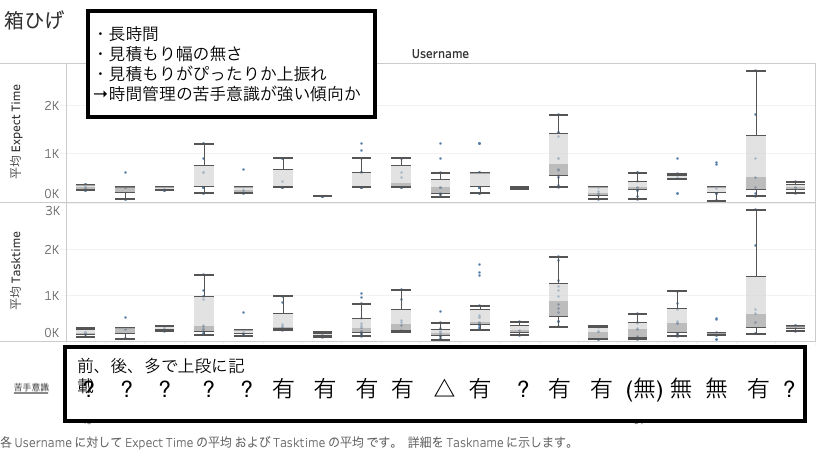
\includegraphics[width=10cm]{images/7/1.png}}
	\caption{3回の計測における見積もりと実測値のずれ(ダミー)}
	\label{fig:hakohige}
	\end{center}
\end{figure}

その上で反復測定分散分析(Repeated Measured ANOVA)を用いて分析したところ,〇〇だった.

また,1回目の計測の結果を元に被験者グループを下記の4つに分類した.(実験結果の四分位数を元に調整)

\begin{table}[htb]
  \begin{center}
  \begin{tabular}{|c|c|c|} \hline
    1 & 大前倒し群 & 予測の方がX分以上長かった群  \\ \hline
    2 & 小前倒し群 & 予測の方がX分未満長かった群  \\ \hline
    3 & 小遅延群 & 実測の方がX分以上長かった群  \\ \hline
    4 & 大遅延群 & 実測の方がX分未満長かった群  \\ \hline 
  \end{tabular}
    \caption{バッファモードの選択分岐}
    \label{tb:buffer}
  \end{center}
\end{table}

その後計測2回分の経過をグループ別に表すとそれぞれ図~\ref{fig:2},~\ref{fig:3},~\ref{fig:4},~\ref{fig:5}の様になった.

\begin{figure}[htb]
\begin{center}
\begin{tabular}{c}

  \begin{minipage}[htb]{\linewidth}
  \begin{center}
  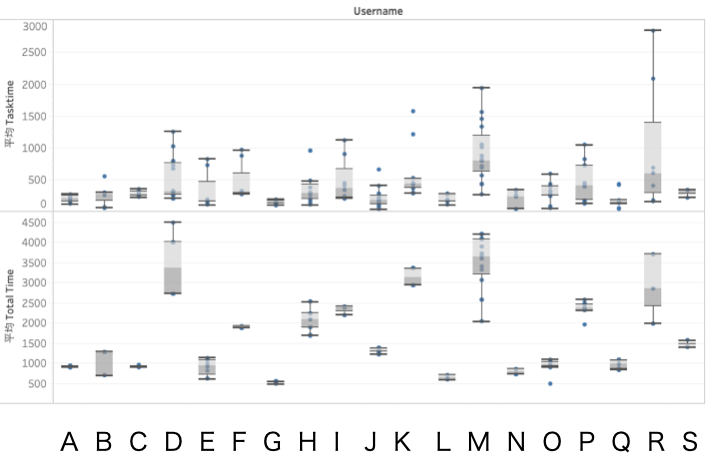
\includegraphics[width=12cm]{images/7/2.png}
  \caption{大前倒し群の推移}
  \label{fig:2}
  \end{center}
  \end{minipage}
  
  \\
  
  \begin{minipage}[htb]{\linewidth}
  \begin{center}
  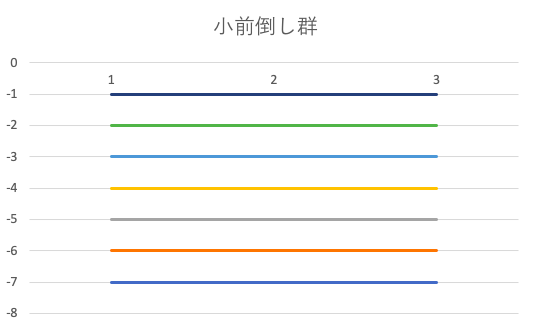
\includegraphics[width=12cm]{images/7/3.png}
  \caption{小前倒し群の推移}
  \label{fig:3}
  \end{center}
  \end{minipage}

\end{tabular}
\end{center}
\end{figure}

\begin{figure}[htb]
\begin{center}
\begin{tabular}{c}

  \begin{minipage}[htb]{\linewidth}
  \begin{center}
  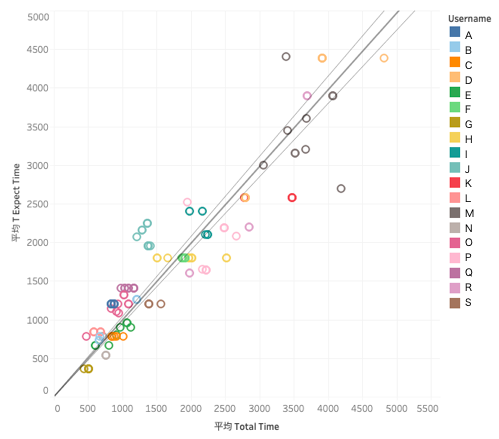
\includegraphics[width=12cm]{images/7/4.png}
  \caption{小遅延群の推移}
  \label{fig:4}
  \end{center}
  \end{minipage}
  
  \\
  
  \begin{minipage}[htb]{\linewidth}
  \begin{center}
  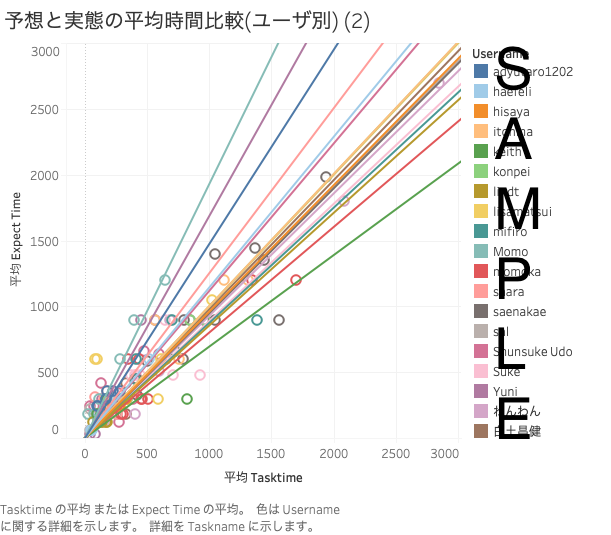
\includegraphics[width=12cm]{images/7/5.png}
  \caption{大遅延群の遷移}
  \label{fig:5}
  \end{center}
  \end{minipage}

\end{tabular}
\end{center}
\end{figure}

\subsection{実験終了後アンケート}

\section{考察}
結果が出次第記述する.

\section{まとめ}
本章では,評価実験にの概要及び手法についてまとめたた上で,結果・考察を述べた.
次章では,本研究における今後の展望と本論文のまとめを述べる.
